\subsection{ALU}

\begin{figure}[H]
\centering
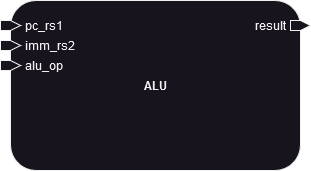
\includegraphics[width=0.75\textwidth]{../diagrams/execute/alu.png}
\caption{Diagram of the ALU}
\label{fig:alu}
\end{figure}

The ALU is a module that is responsible for executing the arithmetic and logic operations. So every mathematical operation is done in this module.

Signals:
\begin{enumerate}[label={\textbullet}]
    \item Input: $a$, This signal is representing the first input of the ALU.
    \item Input: $b$, This signal is representing the second input of the ALU.
    \item Input: $op$, This signal is representing the operation that the ALU will execute.
    \item Output: $out$, This signal is representing the output of the ALU.
\end{enumerate}